
%%%%%%%%%%%%%%%%%%%%%%% file typeinst.tex %%%%%%%%%%%%%%%%%%%%%%%%%
%
% This is the LaTeX source for the instructions to authors using
% the LaTeX document class 'llncs.cls' for contributions to
% the Lecture Notes in Computer Sciences series.
% http://www.springer.com/lncs       Springer Heidelberg 2006/05/04
%
% It may be used as a template for your own input - copy it
% to a new file with a new name and use it as the basis
% for your article.
%
% NB: the document class 'llncs' has its own and detailed documentation, see
% ftp://ftp.springer.de/data/pubftp/pub/tex/latex/llncs/latex2e/llncsdoc.pdf
%
%%%%%%%%%%%%%%%%%%%%%%%%%%%%%%%%%%%%%%%%%%%%%%%%%%%%%%%%%%%%%%%%%%%

% RECOMMENDED %%%%%%%%%%%%%%%%%%%%%%%%%%%%%%%%%%%%%%%%%%%%%%%%%%%
\documentclass{llncs}
% choose options for [] as required from the list
% in the Reference Guide

\usepackage{mathptmx}       % selects Times Roman as basic font
\usepackage{helvet}         % selects Helvetica as sans-serif font
\usepackage{courier}        % selects Courier as typewriter font
\usepackage{type1cm}        % activate if the above 3 fonts are
                             % not available on your system

\usepackage{makeidx}         % allows index generation
\usepackage{graphicx}        % standard LaTeX graphics tool
                             % when including figure files
\usepackage{multicol}        % used for the two-column index
\usepackage[bottom]{footmisc}% places footnotes at page bottom
\usepackage{amsmath,epsfig}
\usepackage{graphicx}
\usepackage{palatino,epsfig,latexsym}
\usepackage{algorithm}
\usepackage{algorithmic}
\usepackage{amsmath,amsfonts,amssymb,color}
\usepackage{graphicx}
\usepackage{subfigure}
\usepackage{multirow}
\usepackage{bbm}
\usepackage[T1]{fontenc}
\renewcommand{\textfraction}{.01}
\renewcommand{\bottomfraction}{.99}
\renewcommand{\topfraction}{.99}

\usepackage{url}
\newcommand{\keywords}[1]{\par\addvspace\baselineskip
\noindent\keywordname\enspace\ignorespaces#1}
%%%%%%%%%%%%%%%%%%%%%%%%%%%%%%%%%%%%%%%%%%%%%%%%%%%%%%%%%%%%%%%%%%%%%%%%%%%%%%%%%%%%%%%%%

\begin{document}
\sloppy
%\mainmatter  % start of an individual contribution
\title{Studying browser-based distributed
  evolutionary computation: tolerance and robustness}

\titlerunning{Studying browser-based distributed
  evolutionary computation: tolerance and robustness }

\author{S. E. Veral \inst{1} \and A. U. Thors \inst{2}}
\institute{ U. Here 
\and
R. U. There}

% \author{Mario Garc\'ia-Valdez\inst{1} \and Leonardo Trujillo\inst{1} \and  Francisco Fern\'andez de Vega\inst{2} \and
% Juan J. Merelo Guerv\'os\inst{3} \and Gustavo Olague\inst{4}}

% \institute{Instituto Tecnol\'ogico de Tijuana, Tijuana BC, Mexico
% \and
% Grupo de Evoluci\'on Artificial, Universidad de Extremadura, M\'erida, Spain
% \and
% Universidad de Granada, Granada, Spain
% \and
% Centro de Investigaci\'on Cient\'ifica y de Educaci\'on Superior de Ensenada,\\ Ensenada BC, Mexico\\
% \email{mario@tectijuana.edu.mx,leonardo.trujillo@tectijuana.edu.mx}\\
% \email{fcofdez@unex.es,jmerelo@geneura.ugr.es,olague@cicese.mx}}

% \authorrunning{Garc\'ia-Valdez et al.}

\maketitle


\begin{abstract}
In this paper we explore the computational capabilities of EvoSpace, a
cloud service  that hosts evolutionary algorithms and is based on the
tuple space model, an associatively addressed memory space shared by
several processes, in this case hosted in browsers; these browsers
running JavaScript, acting as clients and called EvoWorkers, connect
to EvoSpace and periodically take a subset of individuals from the
global population, 
perform evolutionary operations on them, and return a set of new
individuals. Several EvoWorkers carry out the evolutionary search in
parallel and asynchronously, interacting with each other through the
central repository. EvoSpace has been tested in the past on several
problems using more or less conventional set ups; in this case we
explore its capabilities in two different directions: using realistic
assumptions of browsers dropping out of the experiment and, on the
other hand, using the multitude of clients to run different versions
of the parameter space.

% Habr�a que decir algo de las conclusiones.

\keywords{Distributed Evolutionary Algorithms, Tuple Space, Cloud
  Computing, }
\end{abstract}


\section{Introduction}
\label{sec:intro}

% Habr�a que reescribirlo... 
Currently, computational resources are offered as different types of services within the Cloud computing model (CCM) \cite{cloud}.
For example, infrastructure as a service (IaaS) such as Amazon's EC2, or Platform as a Service (PaaS) such as Google's App Engine.
However, within Evolutionary Computation (EC), most algorithms have not been ported to the CCM.
The standard are local, serial and synchronized algorithms, instead of distributed, parallel and asynchronous systems.
Therefore, new proposals that exploit the CCM would be an important contribution within the field,
since it lends itself to models of evolution that can encourage population dynamics not present in standard algorithms.
%Moreover, evolutionary systems based on CCM could distribute costly function evaluations over multiple clients.

This paper presents EvoSpace, a population store for the development of evolutionary algorithms (EA) that are intended to run on the Cloud.
Within the CCM, EvoSpace is conceived as a Platform as a Service (PaaS) component, where users can create populations of individuals on demand
without the need to install software or invest in additional hardware.
EvoSpace is designed to be versatile, since the system that manages the population is decoupled from any particular EA.
Client processes, called EvoWorkers, dynamically and asynchronously interact with the EvoSpace store and perform the required evolutionary routines.
EvoWorkers can reside on remote clients or on the platform server. Software as a Service (SaaS) applications could also be developed using EvoSpace, where users could run entire experiments on the Cloud or implement interactive applications that are completely hosted by the service (see \cite{musart2013}).
EvoSpace is well suited for this kind of environment, since it can be accessed by any web enabled device and is robust to lost connections with remote clients. Figure \ref{fig:cloud} presents a conceptual diagram of how EvoSpace fits within the CCM.

\begin{figure*}[t]
    \centering
        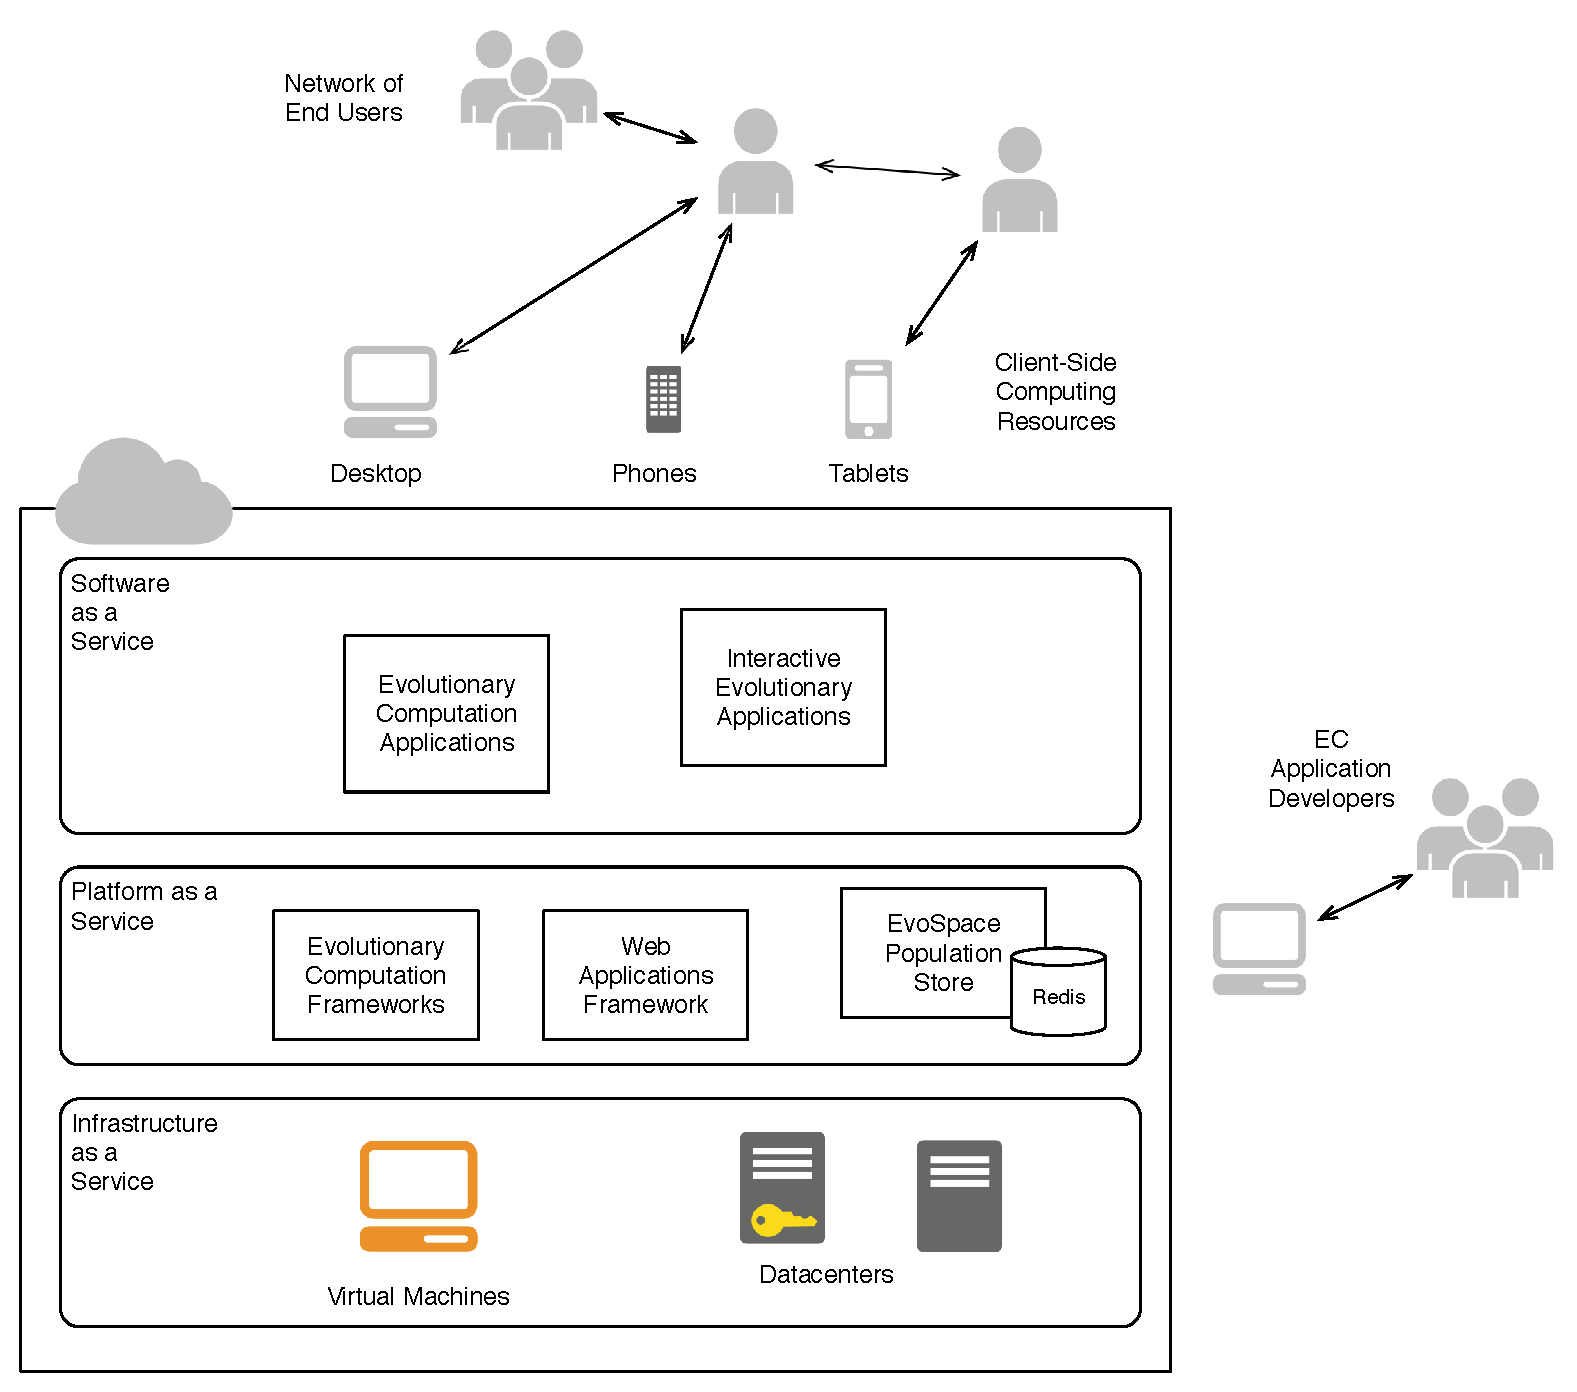
\includegraphics[width=12cm]{cloud2.eps}
    \caption{Conceptual diagram of the CCM and of how EvoSpace can fit within, using it as a PaaS or possible using it to develop a SaaS.}
    \label{fig:cloud}
\end{figure*}

This work presents a proof of concept implementation of EvoSpace. EvoSpace is tested on standard benchmark problems for genetic algorithms, analyzing performance, efficiency and diversity. The remainder of the paper proceeds as follows.Section \ref{sec:work} reviews related work.Afterwards, Section \ref{sec:evo} describes the EvoSpace platform and implementation details.The experimental work is presented in Section \ref{sec:experiments}.Finally, conclusions are given in Section \ref{sec:conclusions}.


\section{Related Work}
\label{sec:work}
The present work builds on several proposals of distributed and interactive EAs.
Langdon \cite{langdon:2004} proposed a distributed EA of artificial agents expressed as fractal structures.
That work employs a global population residing on a central web server that distributes portions of the population using Javascript.
Similar pool-based approaches can be traced back to the A-Teams system \cite{ateam}, which is not restricted to EAs.
Another proposal is made by G. Roy et al. \cite{roy:2009}, who developed a multi-threaded system with a shared memory architecture that is
executed within a distributed environment.
On the other hand, Bollini and Piastra \cite{bollini:1999} emphasize persistence over performance, proposing a system that decouples population storage from the evolutionary operations. A similar model is proposed by Merelo et al. \cite{merelo:2008}, who use a web-server to access a population stored on a database.
Klein and Spector \cite{spector:2007}, and Merelo at al. \cite{merelo:2008}, also propose a Javascript implementations for EAs.
The goal of these papers is to distribute fitness evaluations over the web.
More recently, Cotillon et al. \cite{cotillon:2012} extended browser-based EAs to the Android OS.
The work by Langdon \cite{langdon:2004} is also an interactive EA, where the goal is to evolve virtual creatures.
Similarly, Secretan et al. \cite{picbreeder} and Clune and Lipson \cite{forms}, use web-based interactive EAs to evolve artistic artifacts.
In both cases, user (connected client) collaboration is encouraged.
The most recent comparable work with EvoSpace is the SofEA system of Merelo et al. \cite{sofea1,sofea2}.
SofEA is an EA mapped to a central CouchDB object store.
It provides an asynchronous and distributed search process, where the evolutionary operators are decoupled from the population.
An important difference is that in SofEA all the information regarding the evolutionary progress is continuously updated on the central repository,
while in EvoSpace the population container does not store knowledge regarding the search.


\begin{figure*}[t]
    \centering
        \includegraphics[width=12cm]{evospaceExample.eps}
    \caption{Main components and dataflow within EvoSpace.}
    \label{fig:evo}
\end{figure*}


\section{EvoSpace}
\label{sec:evo}
EvoSpace consists of two main components.
First, the EvoSpace container that stores the evolving population.
The second component consists of the remote clients called EvoWorkers, which
execute the actual evolutionary process, while EvoSpace is only a population repository.
In a basic configuration, EvoWorkers extract a small subset of the population, and use it as the initial population for a local EA executed
on the client machine. Afterwards, the evolved population from each EvoWorker is returned to the EvoSpace container.
The server-side ReInsertionManager process is used to alleviate possible problems that might occur during the search;
for instance, when the EvoSpace container starves or connections are lost.
This can be done because a copy of each sample is stored in a priority queue used by ReInsertionManager to re-insert the sample to the central population;
similar to games where characters are respawned after a certain time.
Figure \ref{fig:evo} illustrates the main components and dataflow within EvoSpace.


\paragraph{The EvoSpace container.}
EvoSpace is based on the tuple space model, an associatively addressed memory space shared by several processes.
A tuple space can be described as a distributed shared memory (DSM) abstraction, organized as a \emph{bag} of tuples.
A tuple $t$ is the basic tuple space element, composed by one or more fields and corresponding values.
In this model, the basic operations that a process can perform is to insert or withdraw tuples from the tuple space.

EvoSpace is composed by a set of objects $ES$ and a set of interface methods provided by a central server.
For an EA system, objects correspond to individuals and all their corresponding features and related information.
Objects can be withdrawn, processed and replaced into $ES$ using a specified set of methods.
However, EvoSpace is different from other tuple space implementations in the sense that retrieving and reading objects from ES are random operations.
Individual objects are not of high interest when accessing $ES$.
Therefore, EvoSpace offers the following interface methods.


\textbf{Read(n):} This method returns a random set $A$ of objects from $ES$, with $|A|=n$ and $A\subset ES$, if $n< |ES|$, the method returns $ES$ otherwise.

\textbf{Take(n):} Returns a random set $A$, following the similar logic used for $Read()$.
However, in this case the sequence of $Take()$ operations provide a temporal dimension to the dynamics of set $ES$.
We can define $ES_i$ as the set at the moment of the $i-th$ $Take()$ operation and $A_i$ as the output.
The contents of EvoSapce are then given by $ES_{i+1}= ES_i \setminus A_i$; i.e., the objets taken are effectively removed from $ES$.
The objects taken are also copied to a new set $S_i$ of \emph{sampled objects} and stored
within a temporary collection $\mathcal{S}$ on the server, implemented as a priority queue.
Sets $S_i \in \mathcal{S}$ can then be reinserted to $ES$ if necessary.

\textbf{ReInsert(i):} This method is used to reinsert the subset of elements removed by the $i-th$ $Take()$ operation,
  such that the contents of EvoSpace are now $ES \cup S_i$ if $S_i \in \mathcal{S}$ and $ES$ is left unchanged otherwise.

\textbf{Insert(A):} This method represents the union operation $ES \cup A$.

\textbf{Replace(A,i):} Similar to $Add()$, however set $A$ should be understood as a replacement for
  some $S_i \in \mathcal{S}$, hence $|A| = |S_i|$, but the objects in $A$ can be different (evolved) objects from those in $S_i$.
  Moreover, if $S_i$ exists it is removed from $\mathcal{S}$.
  However, if $S_i$ does not exist this means that a $ReInsert(i)$ operation preceded it, this increases the size of $ES$.

\textbf{Remove(A):} This method removes all of the objects in $A$ that are also in $ES$, in such a way that
  the contents of EvoSpace are now set to $ES \cup (A\cap ES)$.



\paragraph{Individuals.}
As stated above, objects in $ES$ represent individuals in an EA.
Explicitly, the objects in $ES$ are stored as \emph{dictionaries}, an abstract data type that represents a collection
of unique keys and values with a one to one association.
In this case, keys represent specific properties of each object and the values can be of different types, such as
numbers, strings, lists, tuples or other dictionaries.
In the current implementation, the objects in $ES$ are described by the following basic fields.
An \textbf{id} string that represents a unique identifier for each object.
A \textbf{chromosome} string, which depends on the EA and the representation used.
The \textbf{fitness} dictionary for each individual; allowing the system to store multiple fitness values for multi-objective or dynamic scenarios.
A \textbf{parents} dictionary with identifiers of the individual(s) from which it was produced.
Finally, a \textbf{GeneticOperator}  string that specifies the operator that produced it.


\paragraph{The EvoSpace Server Processes.}
%The EvoSpace architecture employs a client-server architecture with a shared memory container.
On the server side, a process called \textbf{EvoSpaceServer} is executed, which creates and activates a new EvoSpace
container object and waits for requests to execute interface methods.
Additionally, on the server three more processes are executed, these are: \textbf{InitializePopulation}, \textbf{ReInsertionManager} and \textbf{EvolutionManager}.
\textbf{InitializePopulation} is executed once, its goal is obvious, initialize the population by adding $popsize$ random
individuals. The function that creates new individuals depends on the problem and representation used.
\textbf{ReInsertionManager} is used as a failsafe process that periodically checks (every $wt$ seconds) if the size of the population in $ES$
falls below a certain threshold or if the time after the last $ReInsert()$ is greater than $next_r$.
If any of these conditions are satisfied, then $rn$ subsets $S_i \in \mathcal{S}$ are reinserted into ES using the $ReInsert()$ method.
Moreover, the \textbf{ReInsertionManager} makes a $ReInsert(i)$ call when $EvoWorker_i$ (see below) looses a connection with the server,
thus recovering the population sample.
Finally, \textbf{EvolutionManager} periodically checks if a termination condition is satisfied, which is checked by the $isOver()$ method.
This method can be implemented according to the needs of the evolutionary search.
For instance, $isOver()$ can check if an optimal solution is found or if a maximum number of
function evaluations have been performed.


\paragraph{The EvoSpace Clients: EvoWorkers.}
The second component of the proposed model are the processes executed on client machines, referred to as \textbf{EvoWorkers}.
Each client loads a process that executes the main code of the EA.
The \textbf{EvoWorker} process is straightforward, it requests a set of objects $A_i$ from the $ES$ container.
Afterwards, the $Evolve()$ function is called where the actual evolutionary cycle is performed.
In this scenario, $A_i$ can be seen as a local population on which evolution is carried out for $g$ generations.
The result of this evolution is then returned and reinserted into $ES$, then the EvoWorker can request a new set from $ES$ and repeat the process.
Otherwise, each EvoWorker could specialize on a particular part of the evolutionary process, such as selection, evaluation or genetic variation;
an approach not taken in the present work.



\paragraph{Implementation.}
%Figure~\ref{fig:evospace} shows a schematic diagram of the proposed architecture and the corresponding information flow with implementation details.
Individuals are stored in-memory, using the Redis key-value database.
Redis was chosen over a SQL-based management system, or other non-SQL
alternatives, because it provides a hash based implementation of sets
and queues which are natural data structures for the EvoSpace
model. For example, selecting a random key from a set has a complexity
of O(1). The logic of EvoSpace is implemented as a python module
exposed as a Web Service using cherrypy and django http
frameworks. The EvoSpace web service can interact with any language
supporting json-rpc or ajax requests. The EvoSpace modules and workers
in JavaScript, JQuery and python are available with a Simplified BSD
License from https://github.com/evoWeb/EvoSpace. 






\section{Conclusions}
\label{sec:conclusions}
EvoSpace proposes a PaaS system for Cloud-based EAs, where the search is carried out as a distributed and asynchronous process.
%The goal of EvoSpace is to facilitate the development of EAs that can be executed on the cloud, in order to
%exploit the different population that are present on such a model.
EvoSpace is tested on a standard GA benchmark.
While the search conducted by an EvoSpace-based EA is fundamentally different from a standard sequential EA,
the search is able to produce competitive results with regards to solution quality.
Moreover, recent work has also shown that EvoSpace can acomodarte a less common type of EA, an interactive system for artistic design \cite{musart2013}.
While initial results are encouraging, future work must evaluate fault tolerance and the effects of different algorithm parameters and settings.
Also, other features will be incorporated to Evospace, such as multiple populations management, authentication, quotas and throttling.
Finally, to contextualize the main strengths and weaknesses of EvoSpace a comprehensive empirical evaluation must be performed with other
benchmark tests, compared with other distributed and web-based EAs.

\subsubsection*{Acknowledgments.}
\begin{small}
% Research supported by DEGEST-ProIFOPEP (Mexico) Research Project 4616.12-P;
% CONACYT (Mexico) Basic Science Research Project No. 178323;
% Regional Government Junta de Extremadura, Consejer\'ia de Econom\'ia-Comercio e Innovaci\'on and FEDER, project GRU09105;
% projects TIN2011-28627-C04-02 and -03 (ANYSELF),
% awarded by the Spanish Ministry of Science and Innovation;
% and project P08-TIC-03903 awarded by the Andalusian Regional Government.
\end{small}

bibliographystyle{splncs}
\bibliography{geneura}

\end{document} 